\documentclass{beamer}
\addtobeamertemplate{navigation symbols}{}{%
\usebeamerfont{footline}%
\usebeamercolor[fg]{footline}%
\hspace{5em}%
Слайд №\insertframenumber
}
\setbeamercolor{footline}{fg=blue}
%\usetheme{Warsaw}

\usepackage[english, russian]{babel}
\usepackage[absolute,overlay]{textpos}

\usepackage{fontspec}
\setmainfont{Times New Roman}
\setsansfont{Times New Roman}
\setmonofont{Consolas}

\usepackage{sudoku}
\usepackage{tikz}
\usepackage{blkarray}
\usepackage{listings}
\lstset{basicstyle=\footnotesize\ttfamily}
\lstset{escapeinside={<@}{@>}}
\usepackage[cache=false]{minted}
\newminted{python}{fontsize=\scriptsize, linenos=false}

\graphicspath{{../images/}}

\title{Решатель судоку по изображению с камеры}
\subtitle{}
\author{А.~А.~Муравцев\inst{1}}

\institute{
\inst{1}
Высшая школа теоретической механики\\
Санкт-Петербургский Политехнический университет Петра Великого
}

\definecolor{new_green}{rgb}{0.20,0.68,0}
\begin{document}

\renewcommand*\sudokuformat[1]{\Large\sffamily#1}

\frame{\titlepage}

\begin{frame}
\frametitle{Структура проекта}
\tableofcontents
\end{frame}

\begin{frame}[fragile]
\frametitle{Структура проекта}
\begin{lstlisting}
sudoku
.
|__<@\textcolor{red}{lib}@>
|  |__image_preprocess.py <@\textcolor{new_green}{(чёрно-белое, разделение на ячейки)}@>
|  |__sudoku_detection.py <@\textcolor{new_green}{(обн-ие поля и линий, расп-ие цифр)}@>
|  |__sudoku_solver.py <@\textcolor{new_green}{(р-ль на основе рекурсивного перебора)}@>
|  |__solver_algorithm_x.py <@\textcolor{new_green}{(решатель на основе алгоритма X)}@>
|__<@\textcolor{red}{ml\_model}@>
|  |__dataset <@\textcolor{new_green}{(датасет с изображениями напечатанных цифр)}@>
|  |__ml_train.py <@\textcolor{new_green}{(код обучения нейросети на основе dataset)}@>
|  |__neural_net_classifier_2.h5 <@\textcolor{new_green}{(обученная нейросеть)}@>
|__<@\textcolor{red}{telegram\_bot}@>
|  |__bot.py <@\textcolor{new_green}{(код бота)}@>
|  |__empty_sudoku_field.png <@\textcolor{new_green}{(изображение с пустыми ячейками)}@>
|__<@\textcolor{red}{frontend}@>
|  |__sudoku_app.py <@\textcolor{new_green}{(запуск графического приложения)}@>
|__<@\textcolor{red}{tests}@>
|  |__sudoku_pytest.py <@\textcolor{new_green}{(тесты)}@>
|__<@\textcolor{red}{main.py}@> <@\textcolor{new_green}{(основной файл с выводом результатов в консоль)}@>
|__<@\textcolor{red}{exploration.py}@> <@\textcolor{new_green}{(для исследования идей)}@>

\end{lstlisting}

\end{frame}


\section{Распознавание и обработка судоку на изображении}
\subsection{Цветное в чёрно-белое}
\begin{frame}
\frametitle{Преобразование в чёрно-белое изображение. OpenCV}
\begin{center}
\begin{tikzpicture}
	\node[inner sep=0pt] (to_black_white) at (0,0) {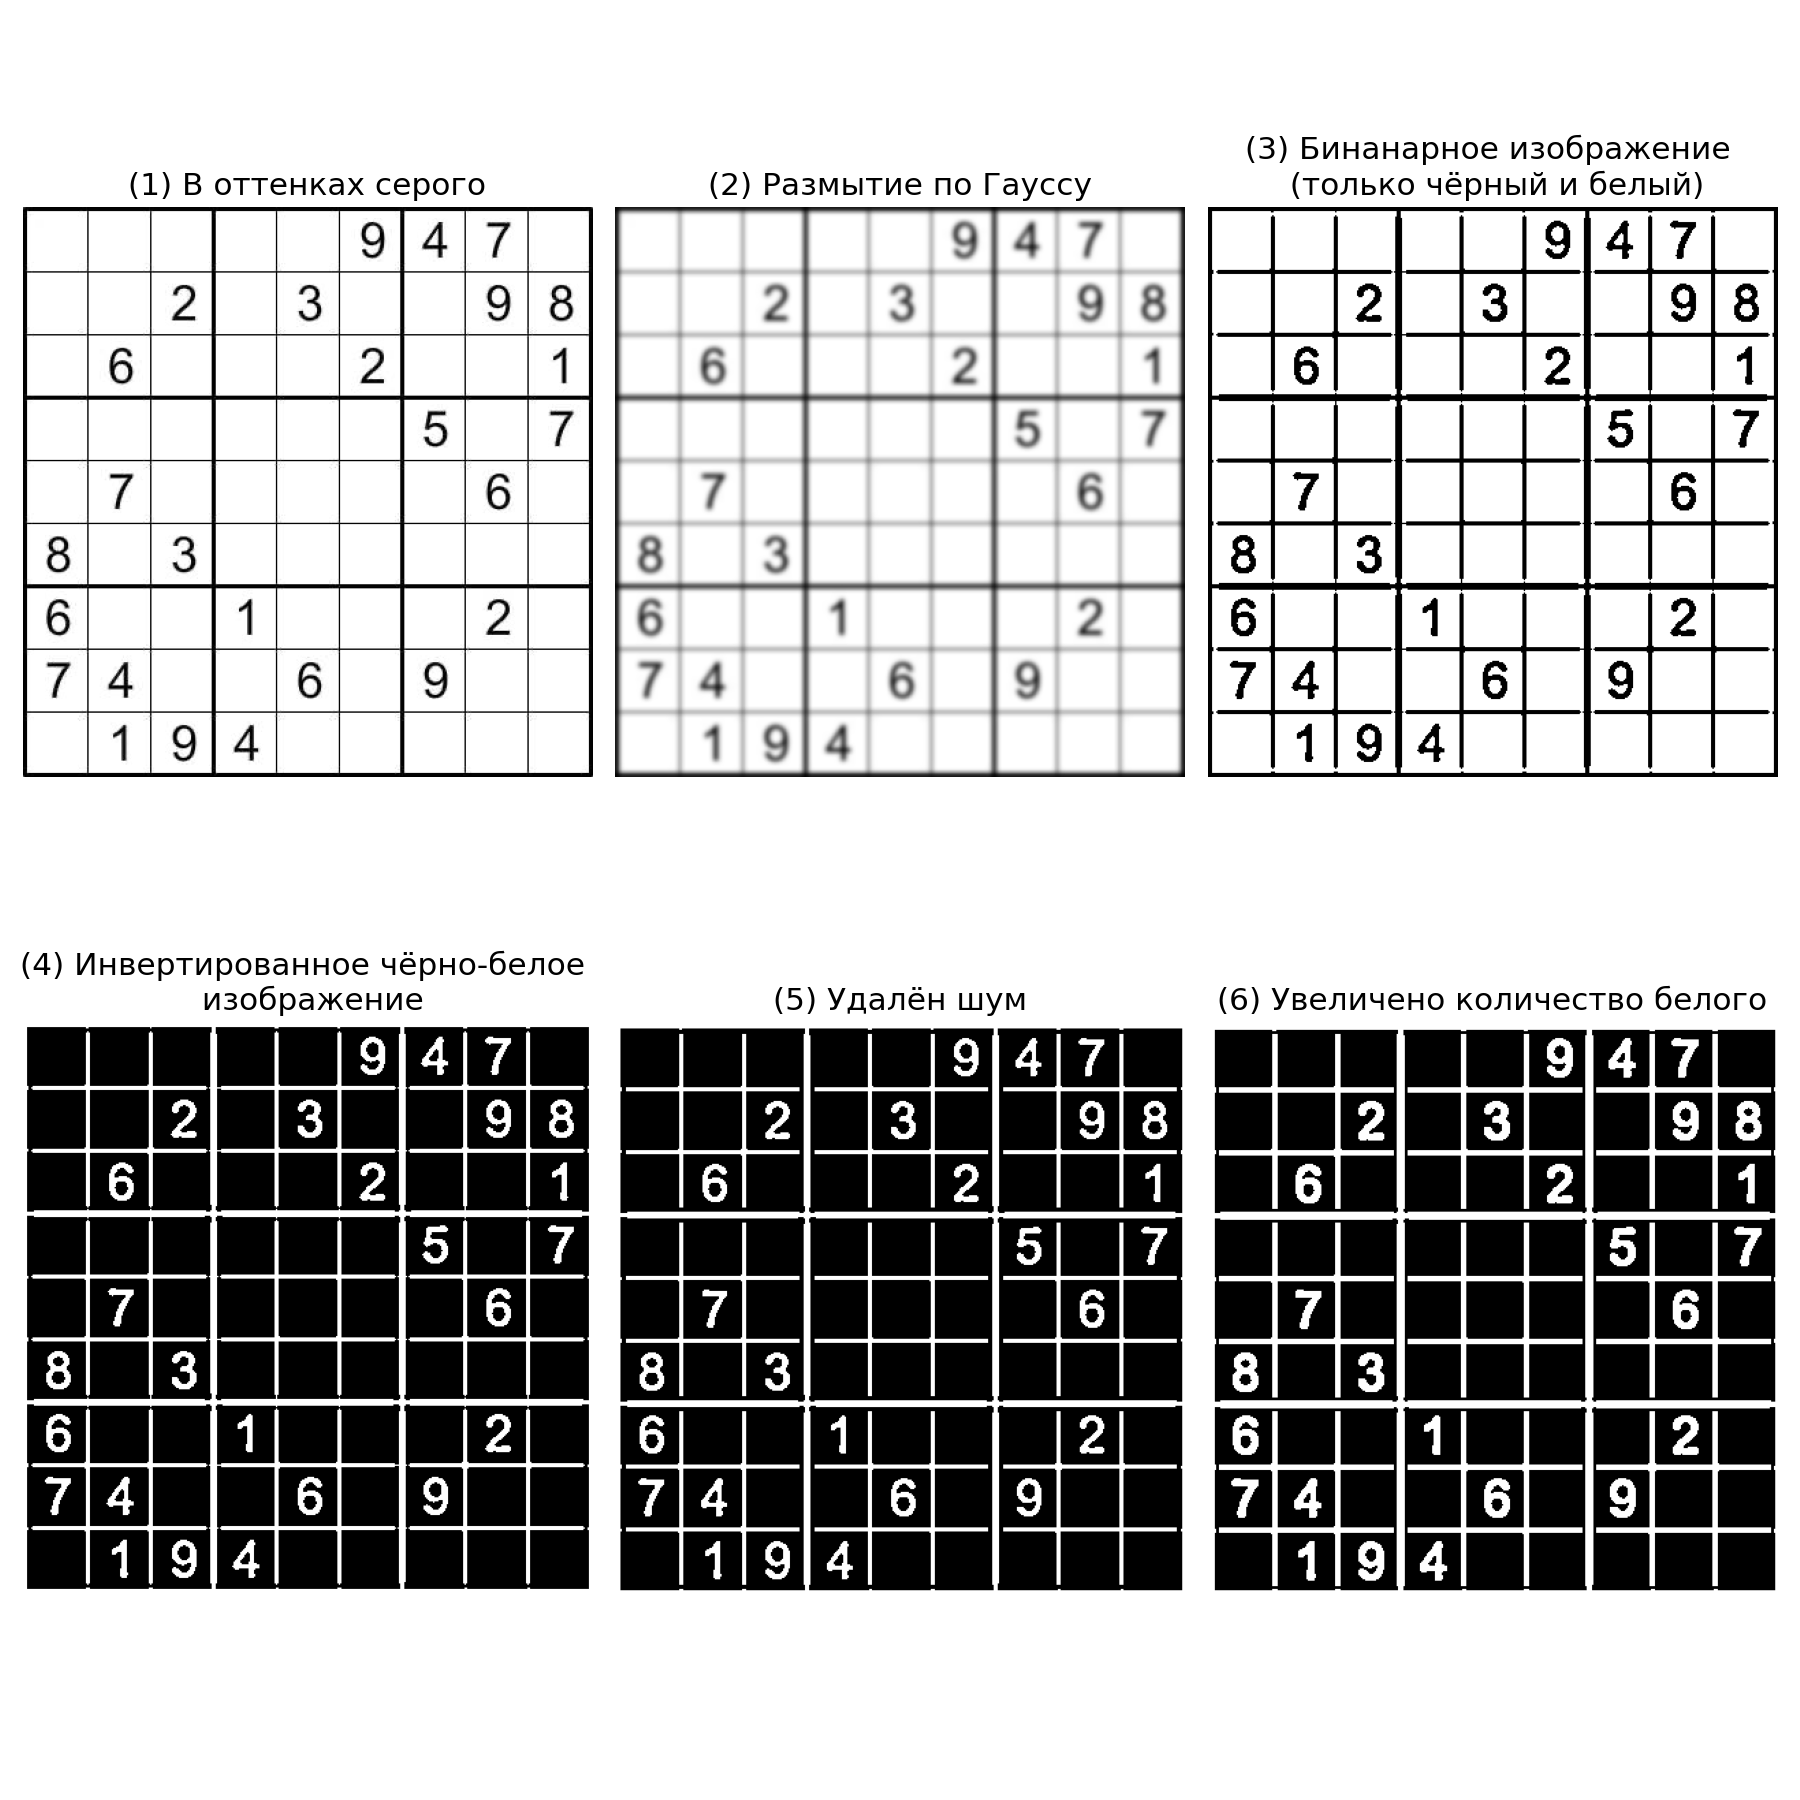
\includegraphics[width=0.7\textwidth]{to_black_white}};
\end{tikzpicture}
\end{center}

\begin{textblock*}{1.5cm}(3cm,1.5cm)
\tiny cv2.cvtColor(...)
\end{textblock*}

\begin{textblock*}{1.5cm}(5.5cm,1.5cm)
\tiny cv2.GaussianBlur(...)
\end{textblock*}

\begin{textblock*}{1.5cm}(8cm,1.5cm)
\tiny cv2.adaptiveThreshold(...)
\end{textblock*}

\begin{textblock*}{1.5cm}(3cm,8.3cm)
\tiny cv2.bitwise\_not(...)
\end{textblock*}

\begin{textblock*}{1.5cm}(5.5cm,8.3cm)
\tiny cv2.morphologyEx(...)
\end{textblock*}

\begin{textblock*}{1.5cm}(8cm,8.3cm)
\tiny cv2.dilate(...)
\end{textblock*}


\end{frame}


\subsection{Определение местоположения поля судоку на кадре}
\begin{frame}
\frametitle{Распознавание поля судоку. Разделение на ячейки}

\setlength\sudokusize{6cm}
\begin{sudoku-block}
| |2| | |3| |9| |7|.
| |1| | | | | | | |.
|4| |7| | | |2| |8|.
| | |5|2| | | |9| |.
| | | |1|8| |7| | |.
| |4| | | |3| | | |.
| | | | |6| | |7|1|.
| |7| | | | | | | |.
|9| |3| |2| |6| |5|.
\end{sudoku-block}

\begin{textblock*}{4.5cm}(7.5cm,2cm)
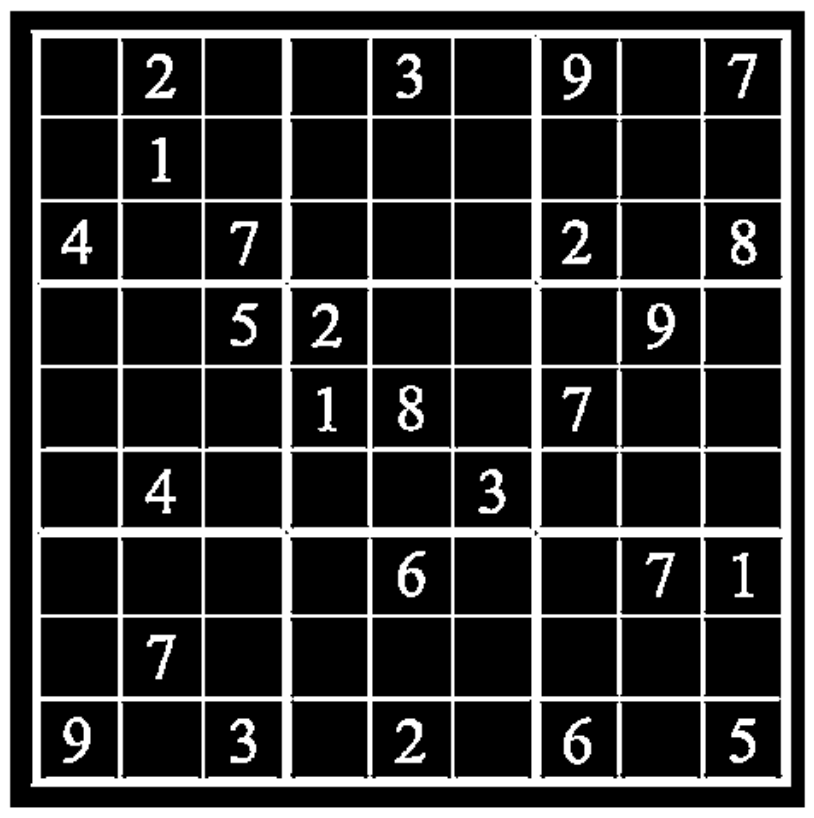
\includegraphics[width=4.5cm]{Sudoku_example6_preprocessed.png}
\end{textblock*}

\begin{textblock*}{4.5cm}(7.7cm,7cm)
\tiny Преобразовано с помощью библиотеки для обработки изображений OpenCV
\end{textblock*}

\end{frame}


\subsection{Распознавание цифр в ячейках с помощью обученной нейронной сети}

\begin{frame}
\frametitle{Датасет}
\begin{textblock*}{10cm}(1cm,1.3cm)
Обычный MNIST не подошёл, так как в нём представлены рукописные, а не напечатанные цифры.
\end{textblock*}

\begin{textblock*}{1.5cm}(1cm,3cm)
\tiny 389 штук

\includegraphics[width=1.5cm]{1_00112}
\end{textblock*}

\begin{textblock*}{1.5cm}(2cm,5cm)
\tiny 412 штук
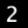
\includegraphics[width=1.5cm]{2_00163}
\end{textblock*}

\begin{textblock*}{1.5cm}(3cm,3cm)
\tiny 388 штук

\includegraphics[width=1.5cm]{3_00108}
\end{textblock*}

\begin{textblock*}{1.5cm}(4cm,5cm)
\tiny 368 штук

\includegraphics[width=1.5cm]{4_00114}
\end{textblock*}

\begin{textblock*}{1.5cm}(5cm,3cm)
\tiny 389 штук

\includegraphics[width=1.5cm]{5_00063}
\end{textblock*}

\begin{textblock*}{1.5cm}(6cm,5cm)
\tiny 349 штук

\includegraphics[width=1.5cm]{6_00059}
\end{textblock*}

\begin{textblock*}{1.5cm}(7cm,3cm)
\tiny 414 штук
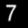
\includegraphics[width=1.5cm]{7_00081}
\end{textblock*}

\begin{textblock*}{1.5cm}(8cm,5cm)
\tiny 367 штук

\includegraphics[width=1.5cm]{8_00068}
\end{textblock*}

\begin{textblock*}{1.5cm}(9cm,3cm)
\tiny 396 штук

\includegraphics[width=1.5cm]{9_00091}
\end{textblock*}

\end{frame}


\begin{frame}
\frametitle{Датасет}
\begin{textblock*}{10cm}(1cm,1.3cm)
Возможны помехи в пустых ячейках: случайный штрих или блик света. При обучении нейросети это 0 (означает пустую ячейку в поле судоку).
\end{textblock*}

\begin{textblock*}{1.5cm}(1cm,3cm)
\tiny пример №1

\includegraphics[width=1.5cm]{0_00032}
\end{textblock*}

\begin{textblock*}{1.5cm}(5cm,3cm)
\tiny пример №2

\includegraphics[width=1.5cm]{0_00116}
\end{textblock*}

\begin{textblock*}{1.5cm}(9cm,3cm)
\tiny пример №3

\includegraphics[width=1.5cm]{0_00118}
\end{textblock*}

\begin{textblock*}{1.5cm}(3cm,5cm)
\tiny пример №4

\includegraphics[width=1.5cm]{0_00010}
\end{textblock*}

\begin{textblock*}{1.5cm}(7cm,5cm)
\tiny пример №5

\includegraphics[width=1.5cm]{0_00021}
\end{textblock*}

\end{frame}

\begin{frame}
\frametitle{Датасет}

\begin{textblock*}{10cm}(1cm,1.3cm)
Возможны и вовсе не случайные помехи: например, просвечивает страница в сборнике судоку.
\end{textblock*}

\begin{textblock*}{4cm}(1cm,3cm)
\tiny Изображение с просвечиванием
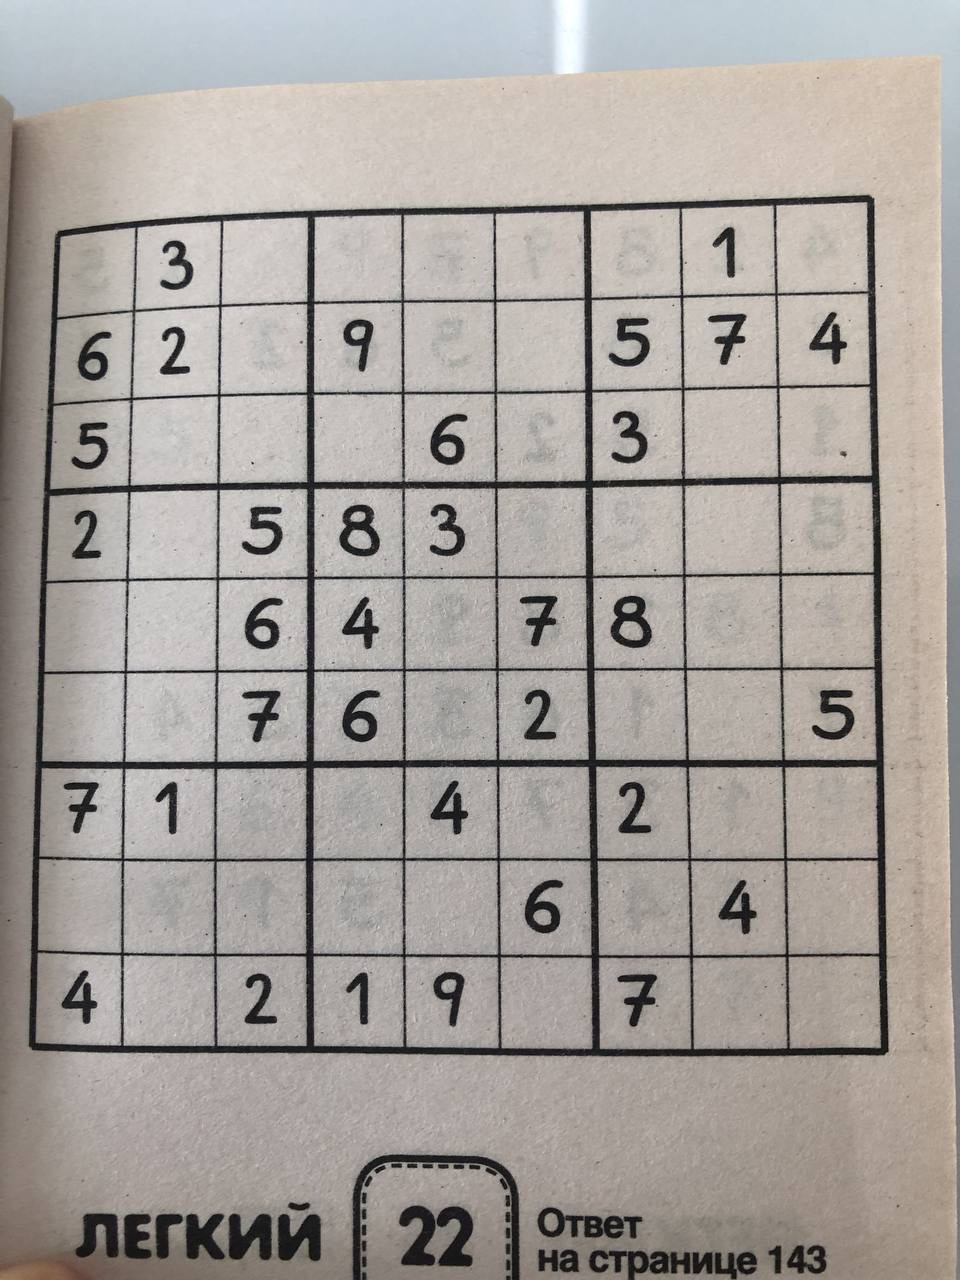
\includegraphics[width=4cm]{sudoku_8_through}
\end{textblock*}

\begin{textblock*}{5cm}(6cm,4cm)
\small При сильном просвечивании нейросеть может уловить паттерн просвечивающей цифры.
\end{textblock*}

\begin{textblock*}{5cm}(6cm,6cm)
\small Дополнительно видим, что есть разные начертания одних и тех же цифр $\Rightarrow$ необходимость расширения датасета.
\end{textblock*}

\end{frame}

\begin{frame}
\frametitle{Свёрточная нейросеть Keras}

\begin{textblock*}{5cm}(3cm,1cm)
\tiny Архитектура
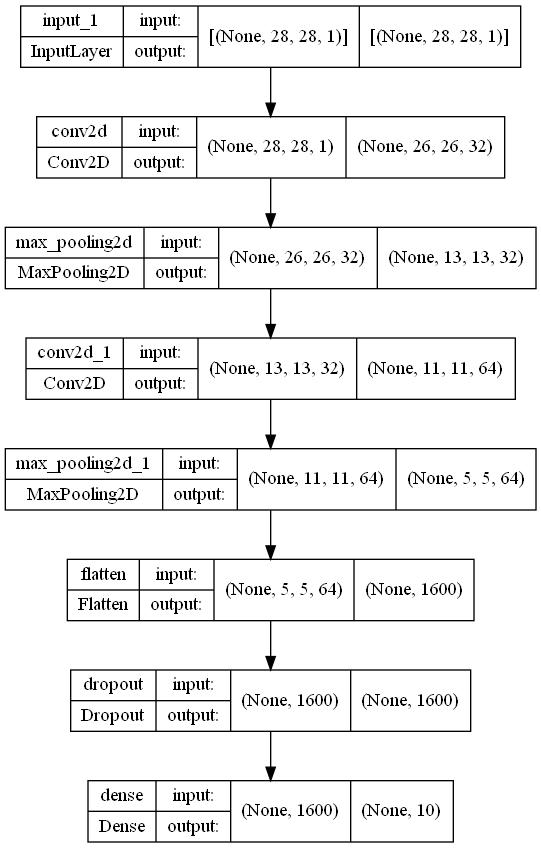
\includegraphics[width=5cm]{model_plot}
\end{textblock*}

\begin{textblock*}{4cm}(8.4cm,1.6cm)
\tiny Входной слой
\end{textblock*}

\begin{textblock*}{4cm}(8.4cm,2.6cm)
\tiny Свёртка
\end{textblock*}

\begin{textblock*}{4cm}(8.4cm,3.6cm)
\tiny Понижение размерности
\end{textblock*}

\begin{textblock*}{4cm}(8.4cm,4.6cm)
\tiny Свёртка
\end{textblock*}

\begin{textblock*}{4cm}(8.4cm,5.6cm)
\tiny Понижение размерности
\end{textblock*}

\begin{textblock*}{4cm}(8.4cm,6.6cm)
\tiny Все значения в многомерной матрице в один вектор
\end{textblock*}

\begin{textblock*}{4cm}(8.4cm,7.6cm)
\tiny Drop-out регуляризация
\end{textblock*}

\begin{textblock*}{4cm}(8.4cm,8.3cm)
\tiny Полносвязный слой. В данном случае вектор из 1600 значений преобразует в вектор только из 10 значений
\end{textblock*}

\end{frame}

\begin{frame}
\frametitle{Обучение нейросети}

\begin{textblock*}{6cm}(0cm,2cm)
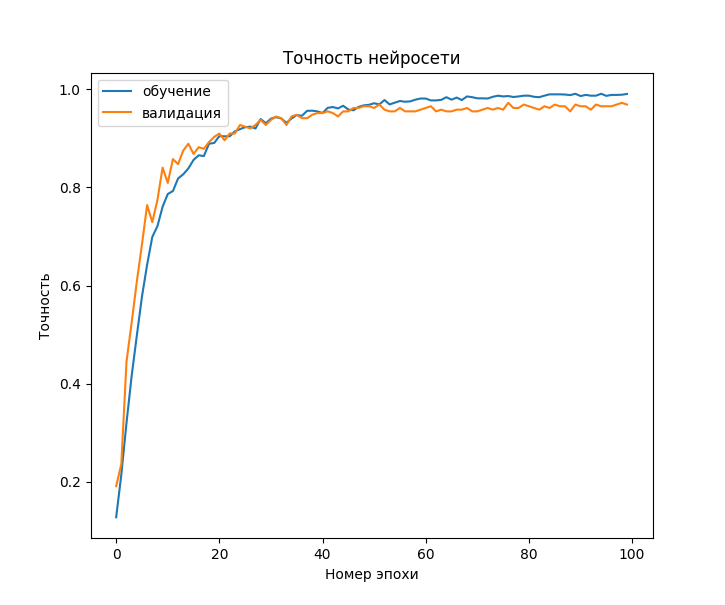
\includegraphics[width=6cm]{model_accuracy}
\end{textblock*}

\begin{textblock*}{6cm}(6cm,2cm)
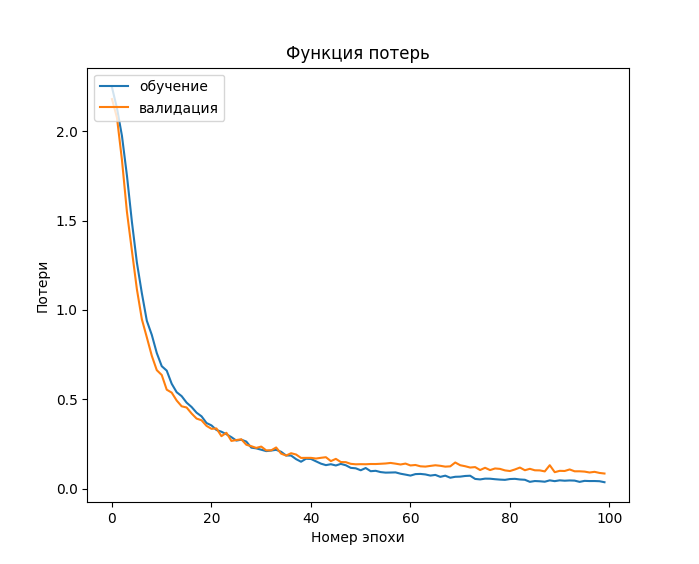
\includegraphics[width=6cm]{model_loss}
\end{textblock*}

\end{frame}

\begin{frame}
\frametitle{Матрица ошибок обученной нейросети}
\begin{textblock*}{10cm}(1cm,1.5cm)
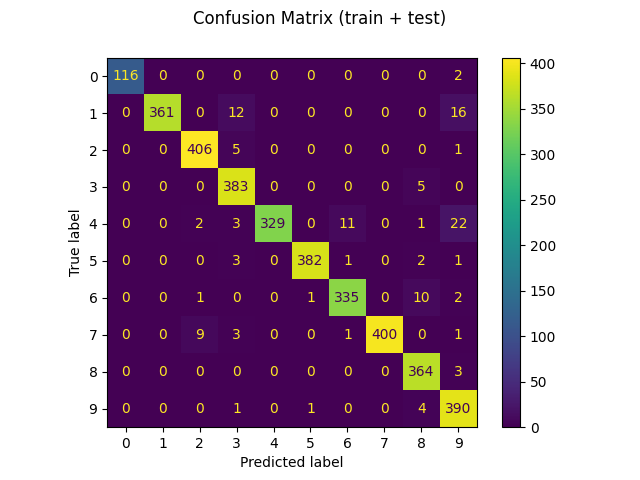
\includegraphics[width=10cm]{net_confusion_matrix}
\end{textblock*}
\end{frame}


\section{Решатель судоку}

\subsection{Рекурсивный перебор}
\begin{frame}
\begin{center}
\frametitle{Рекурсивный перебор, поиск с возвратом (бэктрекинг)}
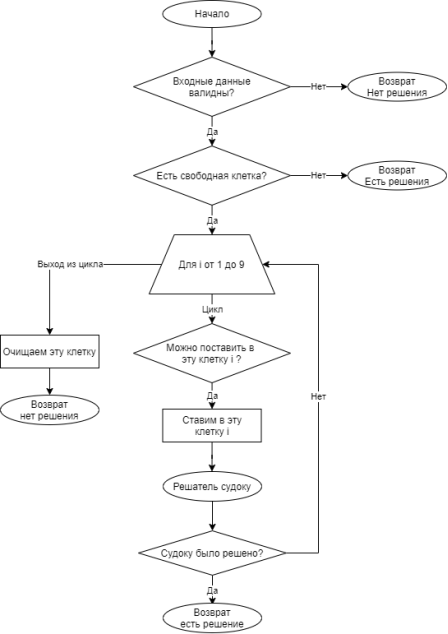
\includegraphics[width=5.5cm]{Sudoku_recursive_scheme}
\end{center}
\end{frame}


\subsection{Постановка задачи о точном покрытии}
\begin{frame}

\frametitle{Задача о точном покрытии}

Дано множество $X$ и другое множество $S$, каждый элемент которого есть подмножество множества $X$. Требуется найти такое подмножество $S^{\,*}$ множества $S$, чтобы каждый элемент из $X$ был ровно в одном элементе выбранного подмножества.\\

Пример.

Пусть $X=\{0,1,2,3,4,5,6,7,8\}$.

Пусть $S=\{A,B,C,D,E\}$, где $A=\{0,1,4,6\}$, $B=\{2,3,5\}$, $C=\{0,4,8\}$, $D=\{0,3,3,4,5,7,8\}$, $E=\{1,6,7\}$.

Тогда $S^{\,*}=\{B,C,E\}$ удовлетворяет поставленным условиям.


\end{frame}


\begin{frame}

\frametitle{Удобное представление данных задачи о точном покрытии}

$X=\{0,1,2,3,4,5,6,7,8\}$\\

$S=\{A,B,C,D,E\}$, где $A=\{0,1,4,6\}$, $B=\{2,3,5\}$, $C=\{0,4,8\}$, $D=\{0,2,3,4,5,7,8\}$, $E=\{2,6,7\}$\\
\ \\

\begin{blockarray}{cccccccccc}
 & 0 & 1 & 2 & 3 & 4 & 5 & 6 & 7 & 8 \\
\begin{block}{c(ccccccccc)}
	A & 1 & 1 & 0 & 0 & 1 & 0 & 1 & 0 & 0 \\
	\textcolor{blue}{B} & \textcolor{blue}{0} & \textcolor{blue}{0} & \textcolor{blue}{1} & \textcolor{blue}{1} & \textcolor{blue}{0} & \textcolor{blue}{1} & \textcolor{blue}{0} & \textcolor{blue}{0} & \textcolor{blue}{0} \\
	\textcolor{blue}{C} & \textcolor{blue}{1} & \textcolor{blue}{0} & \textcolor{blue}{0} & \textcolor{blue}{0} & \textcolor{blue}{1} & \textcolor{blue}{0} & \textcolor{blue}{0} & \textcolor{blue}{0} & \textcolor{blue}{1} \\
	D & 1 & 0 & 1 & 1 & 1 & 1 & 0 & 1 & 1 \\
	\textcolor{blue}{E} & \textcolor{blue}{0} & \textcolor{blue}{1} & \textcolor{blue}{0} & \textcolor{blue}{0} & \textcolor{blue}{0} & \textcolor{blue}{0} & \textcolor{blue}{1} & \textcolor{blue}{1} & \textcolor{blue}{0} \\ 
\end{block}

	
\end{blockarray}

\end{frame}



\begin{frame}

\frametitle{Судоку в терминах задачи о точном покрытии}

\hspace*{-1cm}
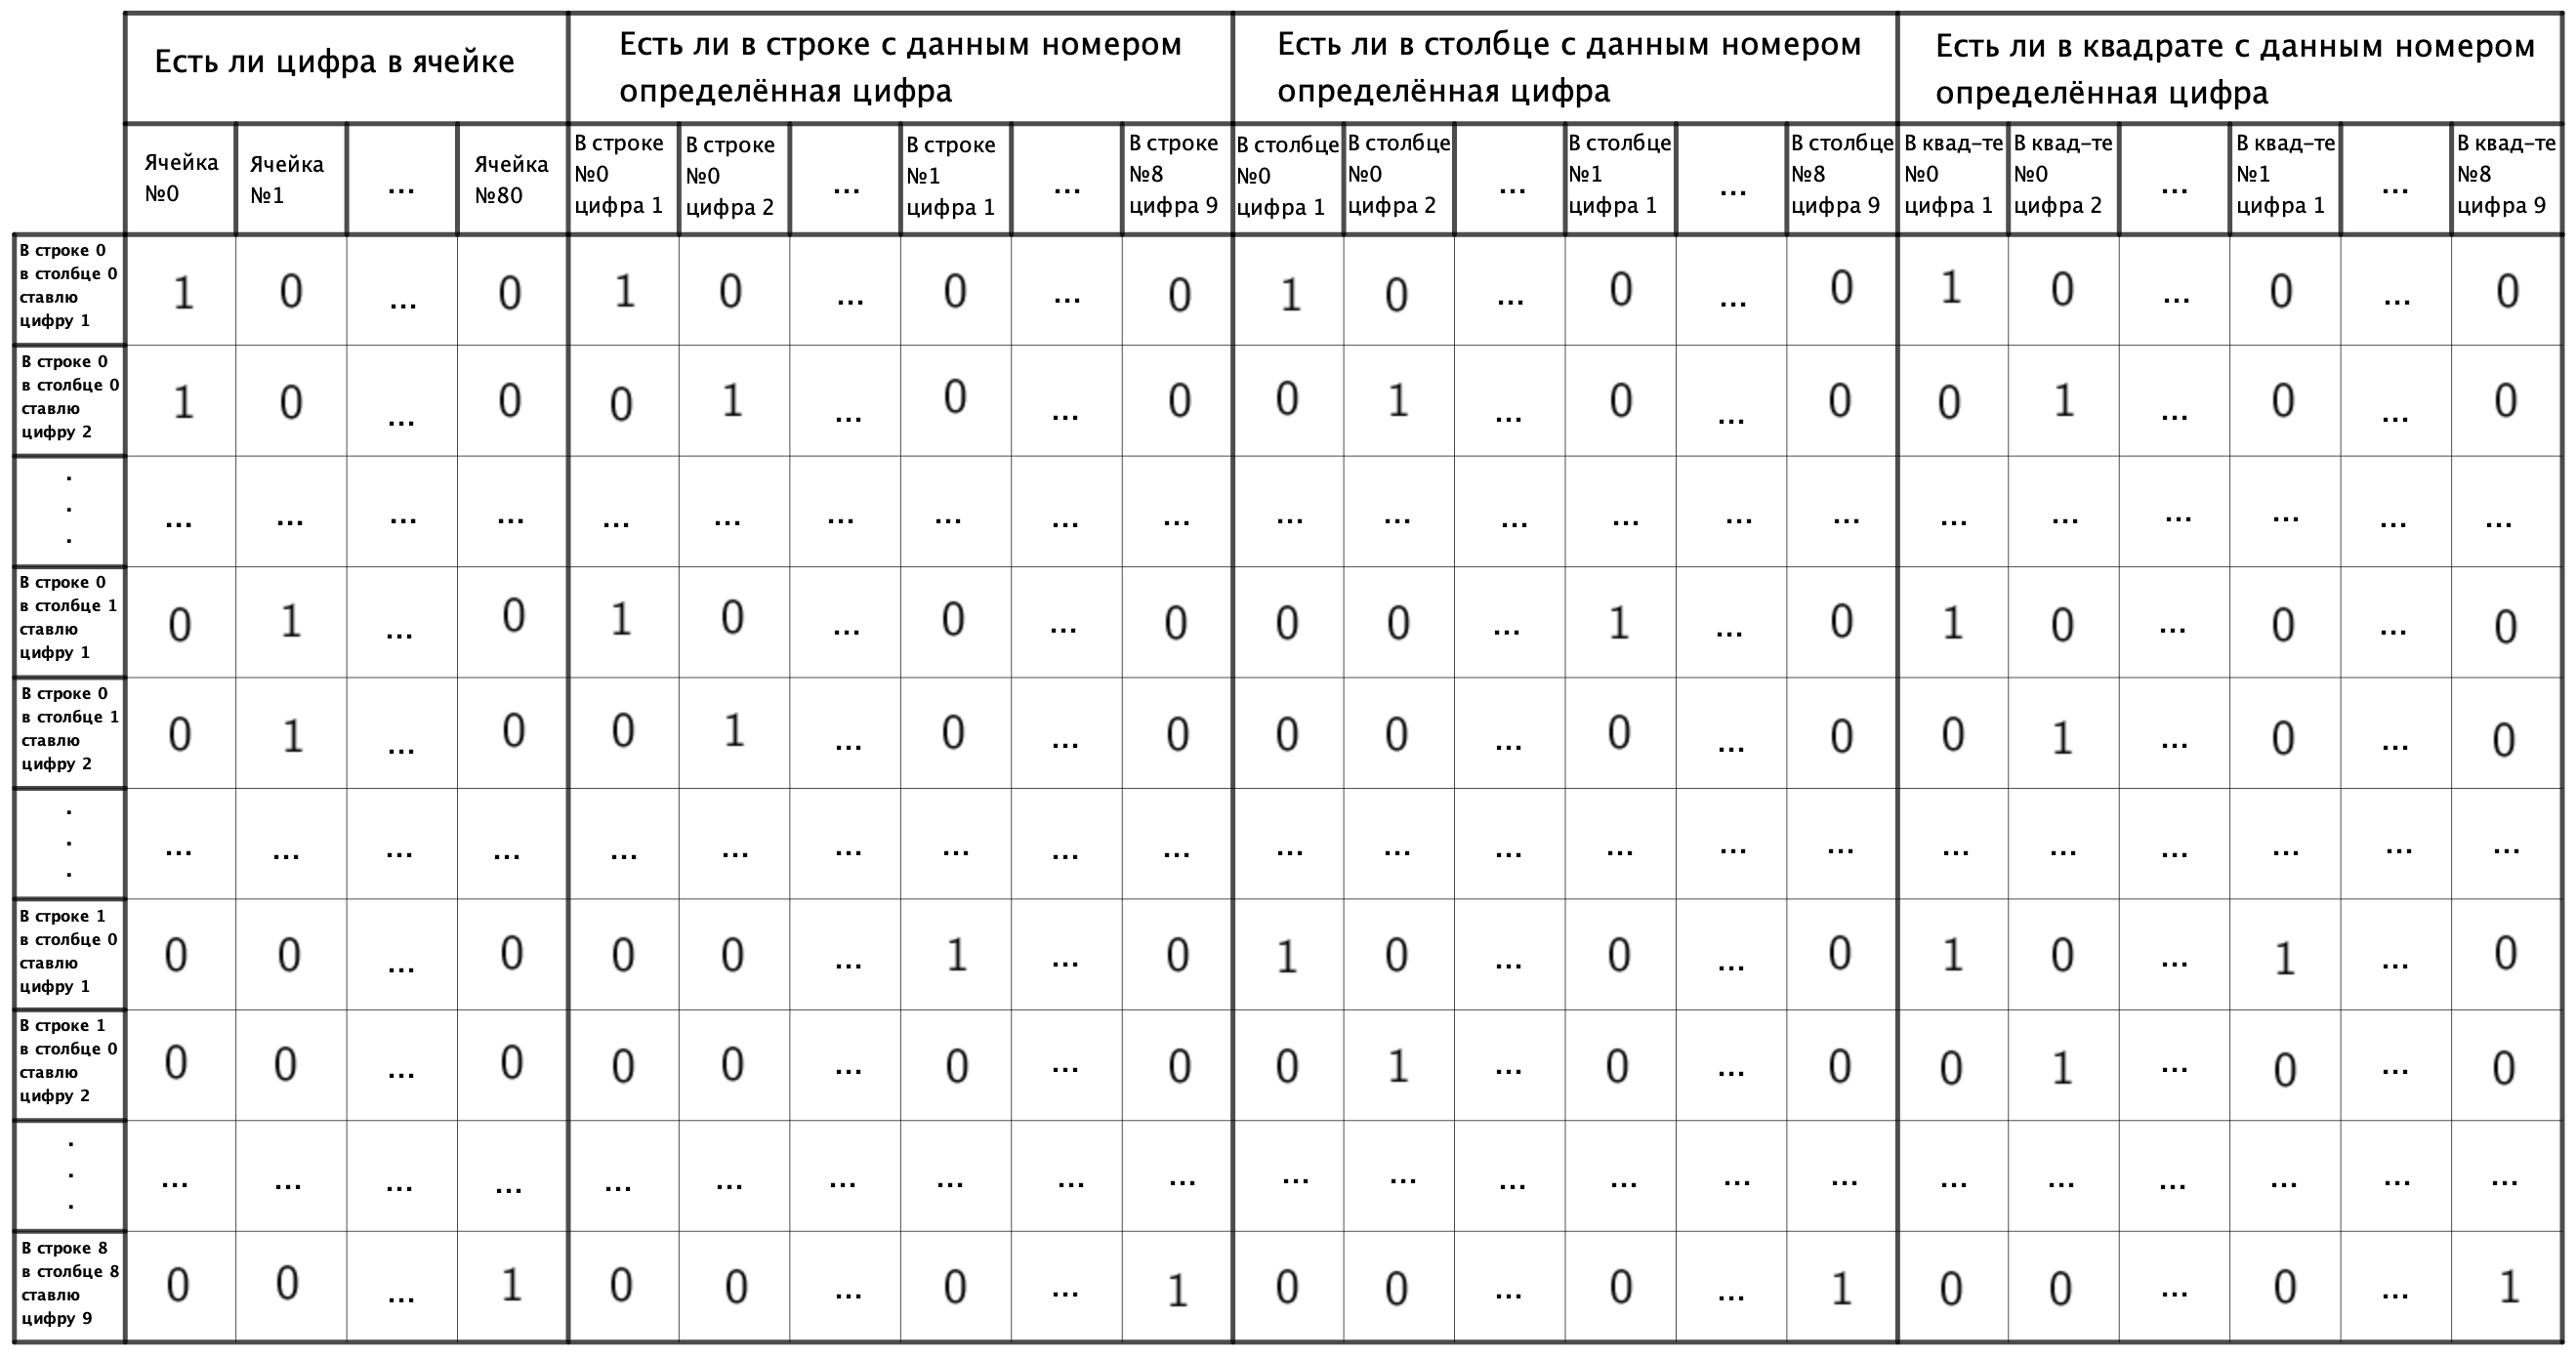
\includegraphics[width=1.15\textwidth]{SudokuToExactCoverProblem}
\begin{textblock*}{7cm}(4.5cm,8.3cm)
729 строк и 324 столбца
\end{textblock*}

\end{frame}


\subsection{Алгоритм X и его реализация с помощью метода танцующих ссылок}
\begin{frame}
\frametitle{Алгоритм X}
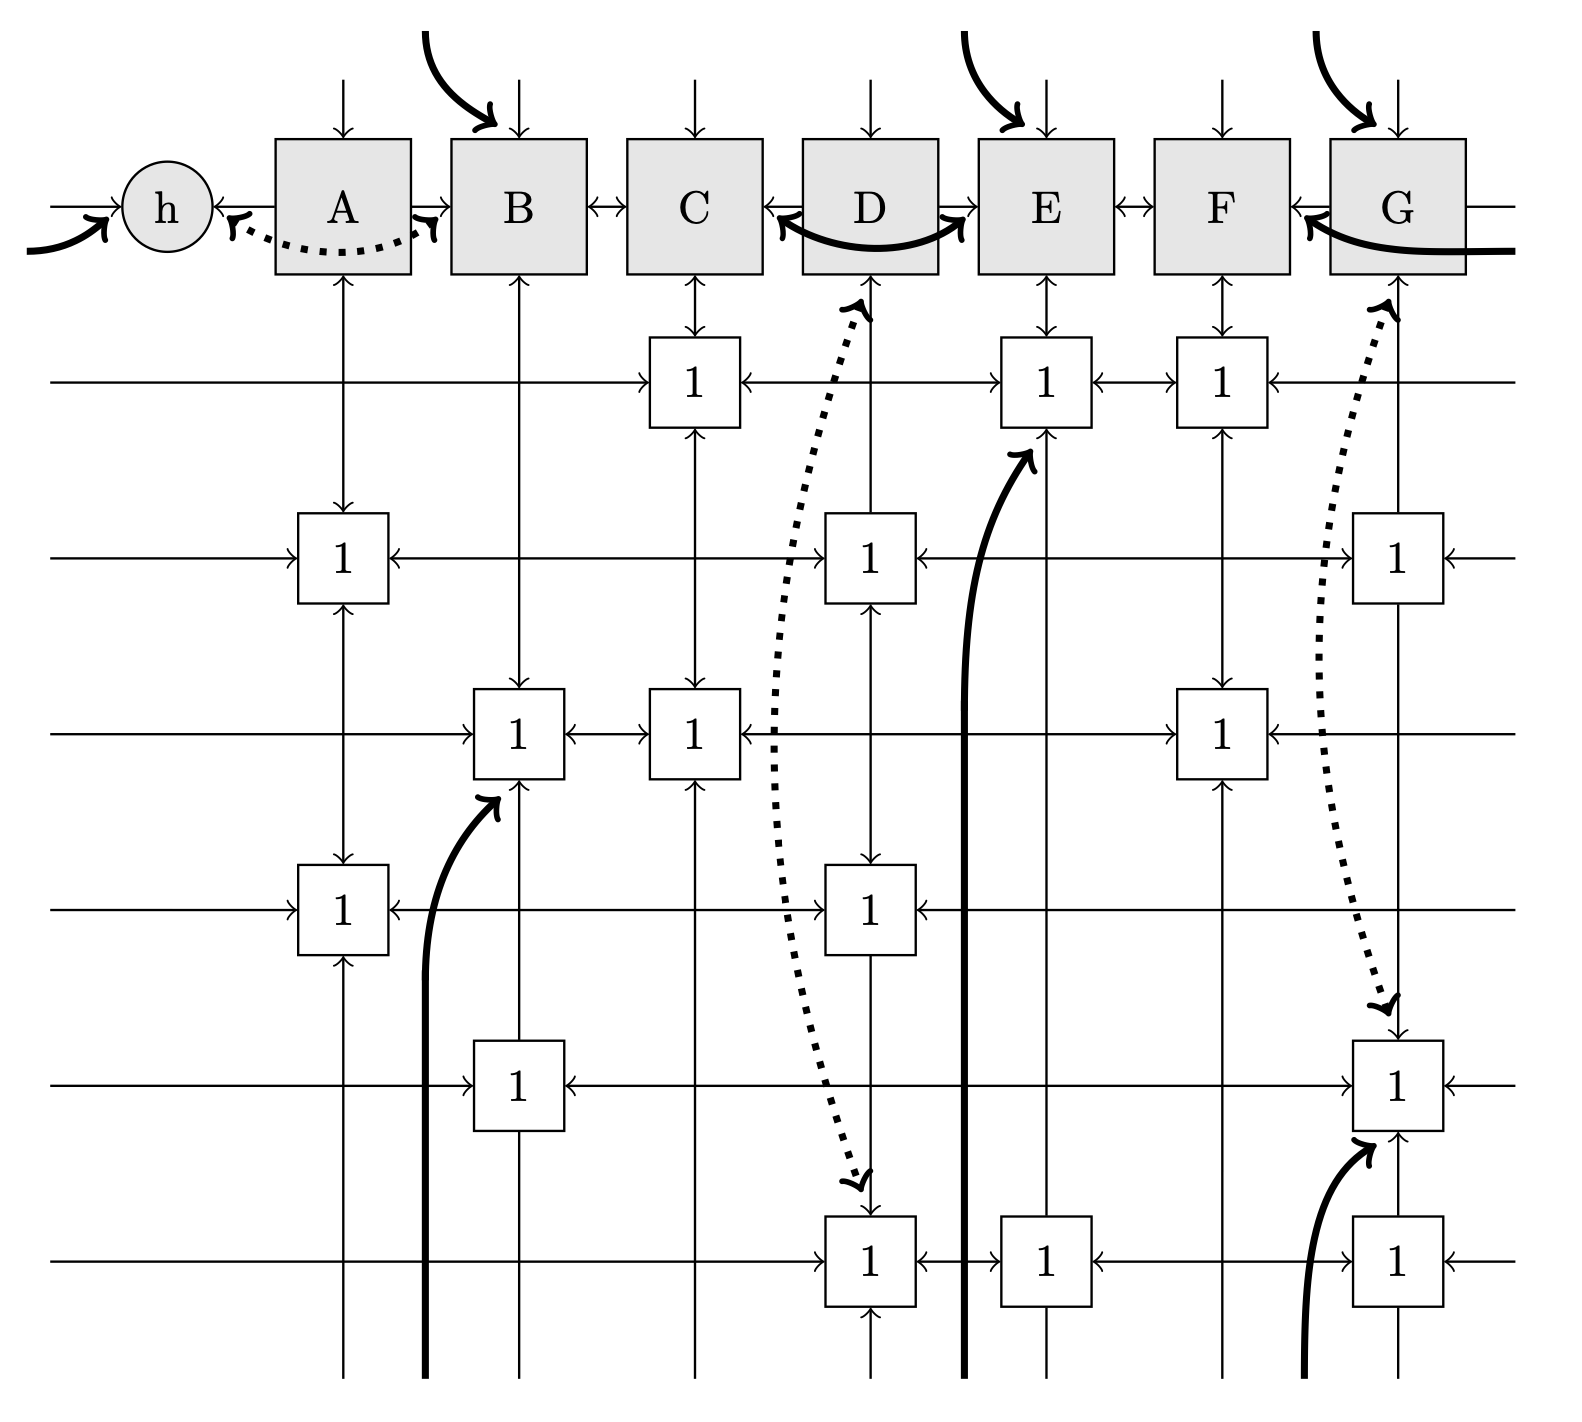
\includegraphics[width=7cm]{algorithmX_example}
\begin{textblock*}{5cm}(8cm,3cm)
Представление бинарной матрицы в виде многосвязного списка
\end{textblock*}

\begin{textblock*}{5cm}(8cm,6cm)
Метод танцующих ссылок
\end{textblock*}


\end{frame}


\section{Телеграм-бот}
\begin{frame}
\frametitle{Телеграм-бот с помощью aiogram}
\begin{textblock*}{5cm}(0cm,1cm)
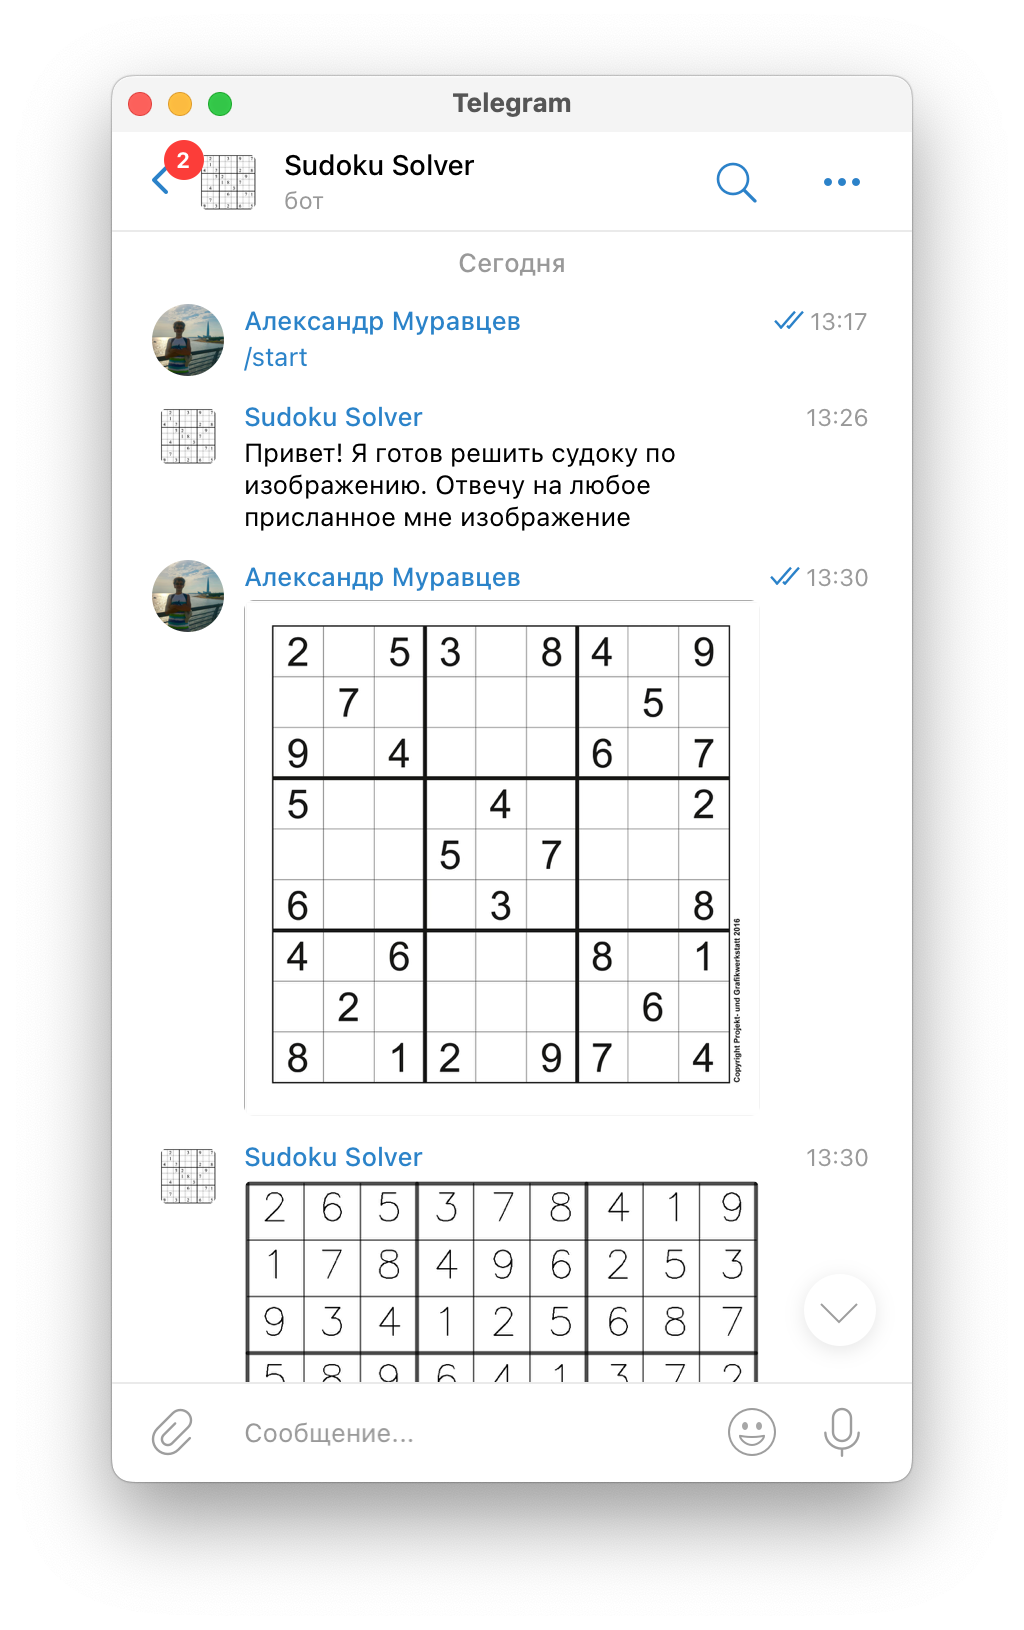
\includegraphics[width=5cm]{telegram_screen_1}
\end{textblock*}

\begin{textblock*}{5cm}(4.5cm,1cm)
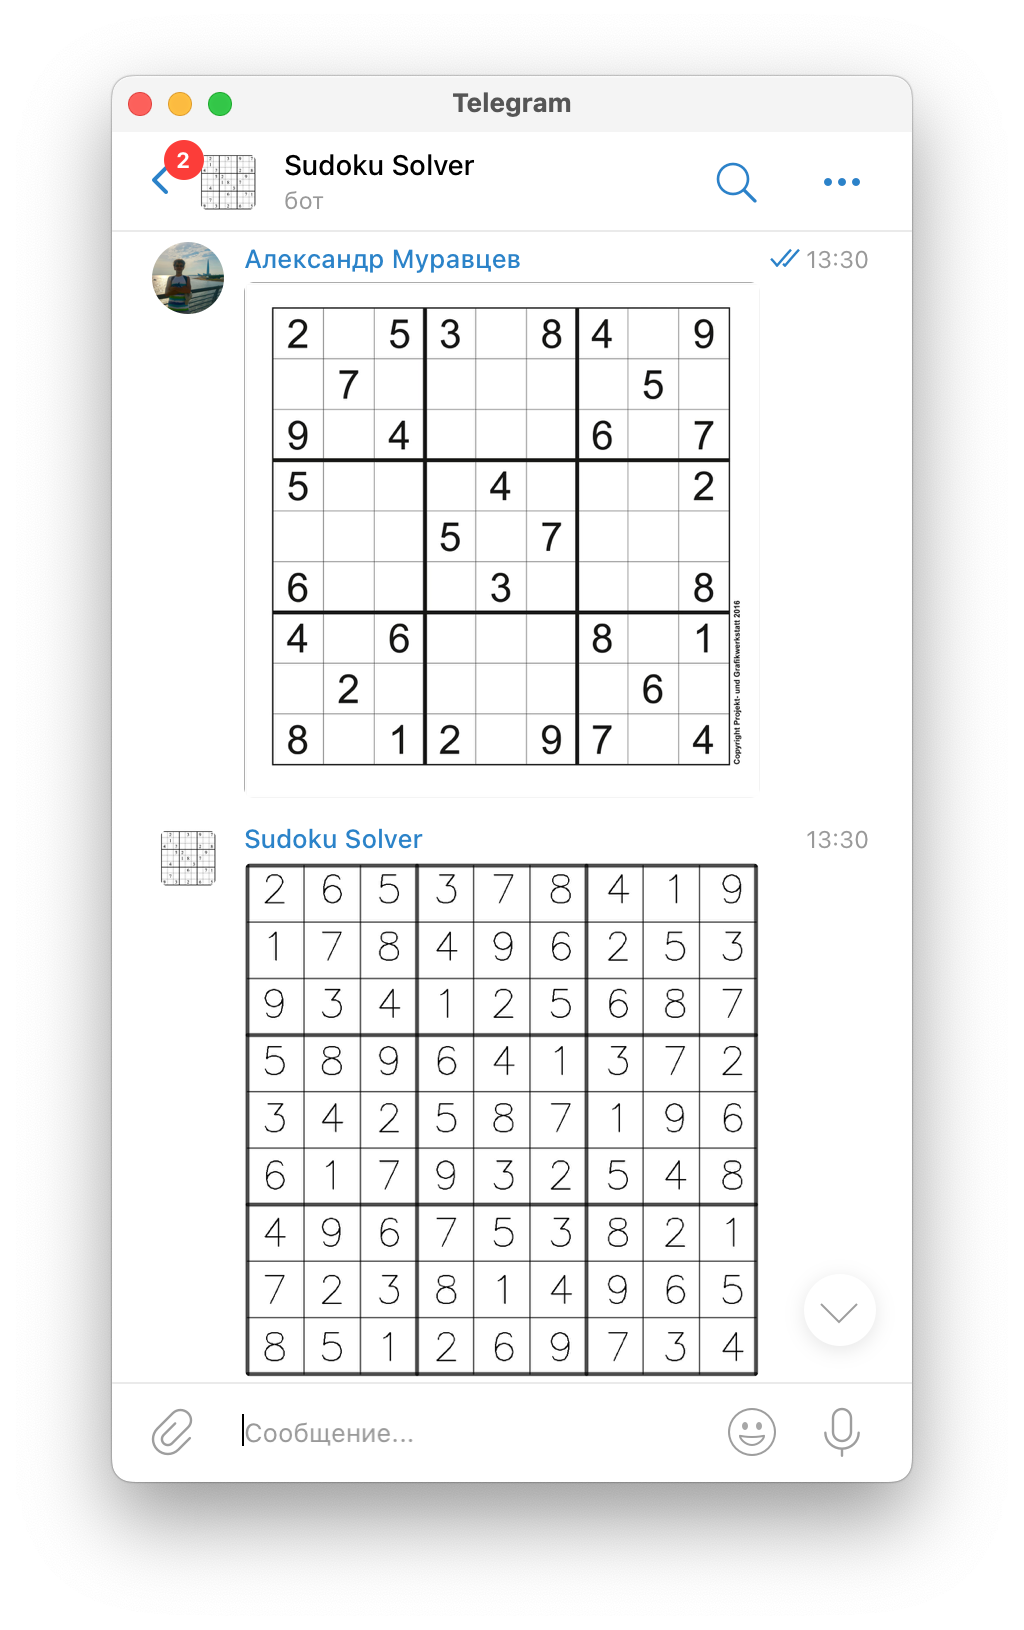
\includegraphics[width=5cm]{telegram_screen_2}
\end{textblock*}

\begin{textblock*}{3cm}(9.3cm,1cm)
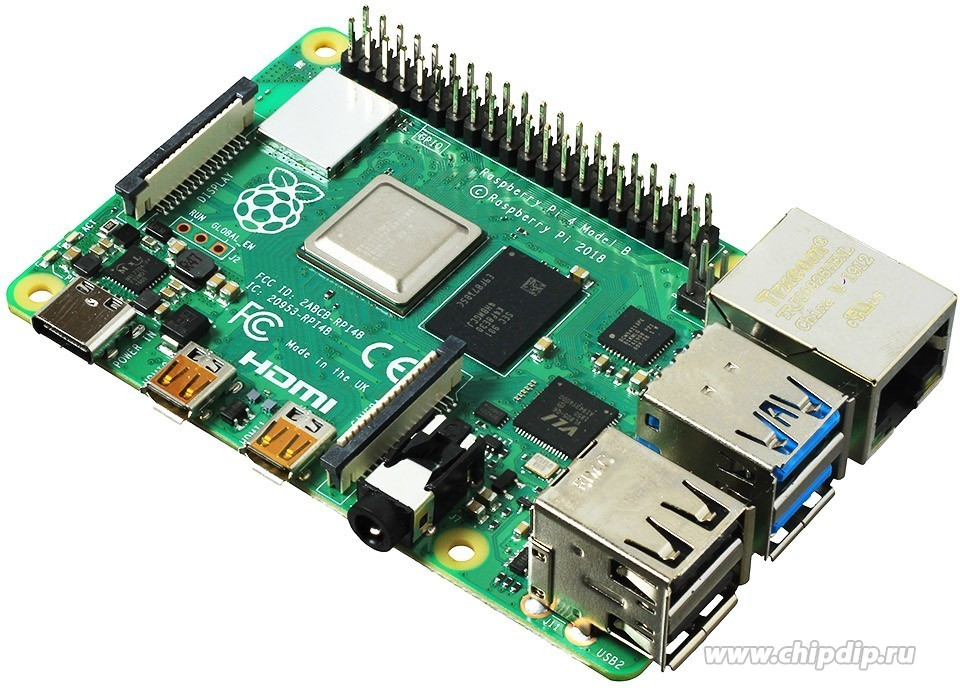
\includegraphics[width=3cm]{Rasberry}
\end{textblock*}

\begin{textblock*}{3cm}(9.3cm,5cm)
\tiny @sudoku\_grids\_solver\_bot

\includegraphics[width=3cm]{qr_frame}
\end{textblock*}

\end{frame}


\begin{frame}
\frametitle{Телеграм-бот}
\begin{textblock*}{5cm}(0cm,1cm)
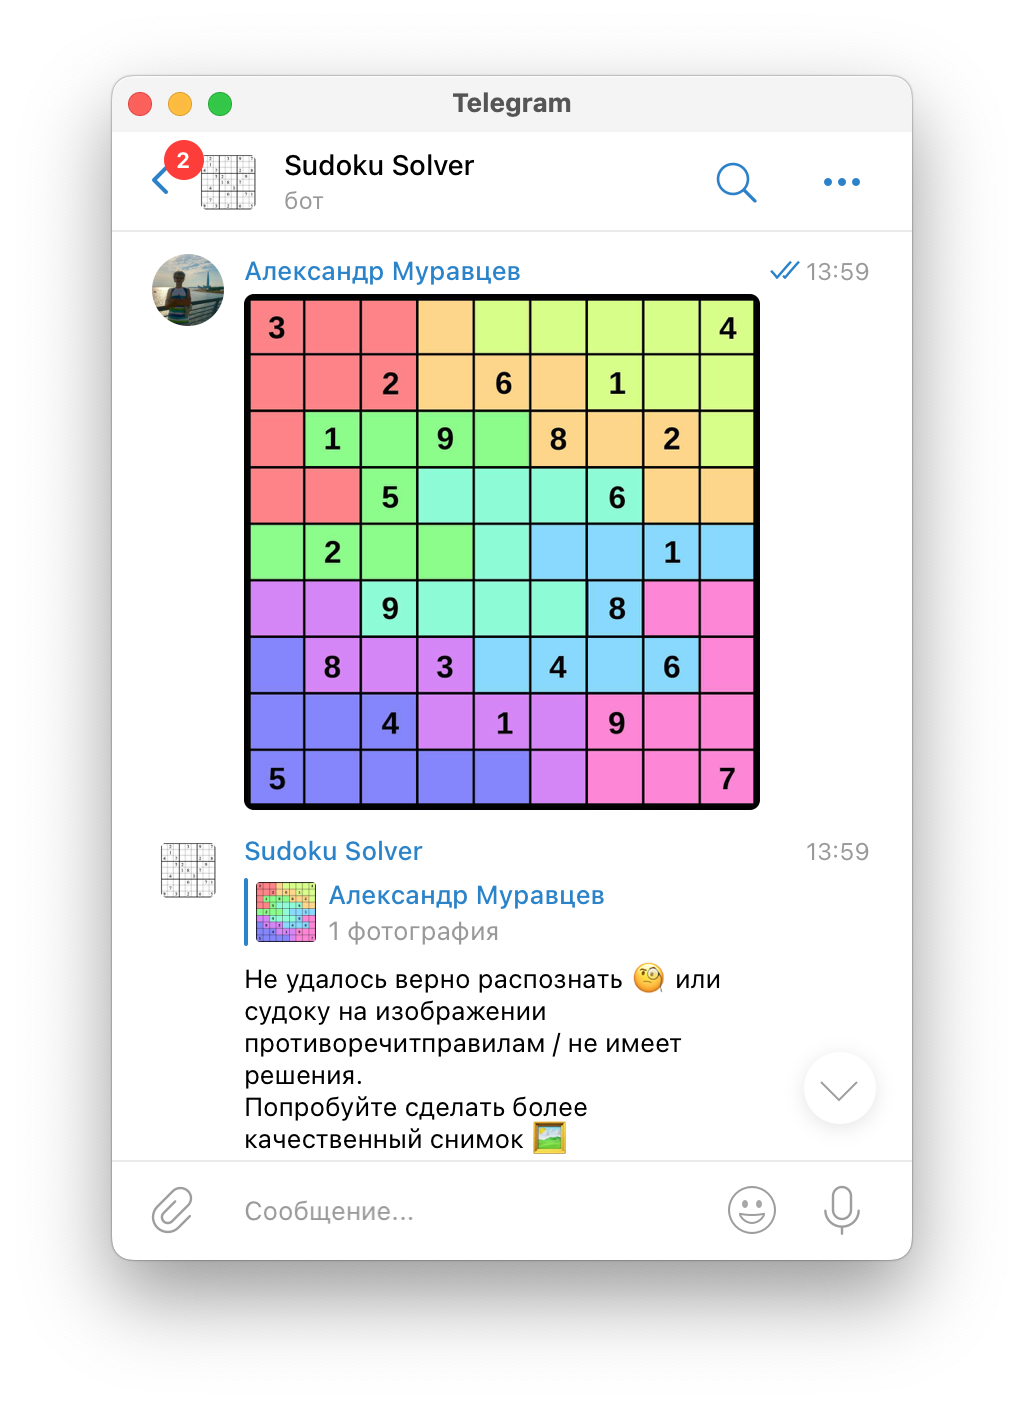
\includegraphics[width=5cm]{telegram_screen_3}
\end{textblock*}

\begin{textblock*}{5cm}(4.1cm,1cm)
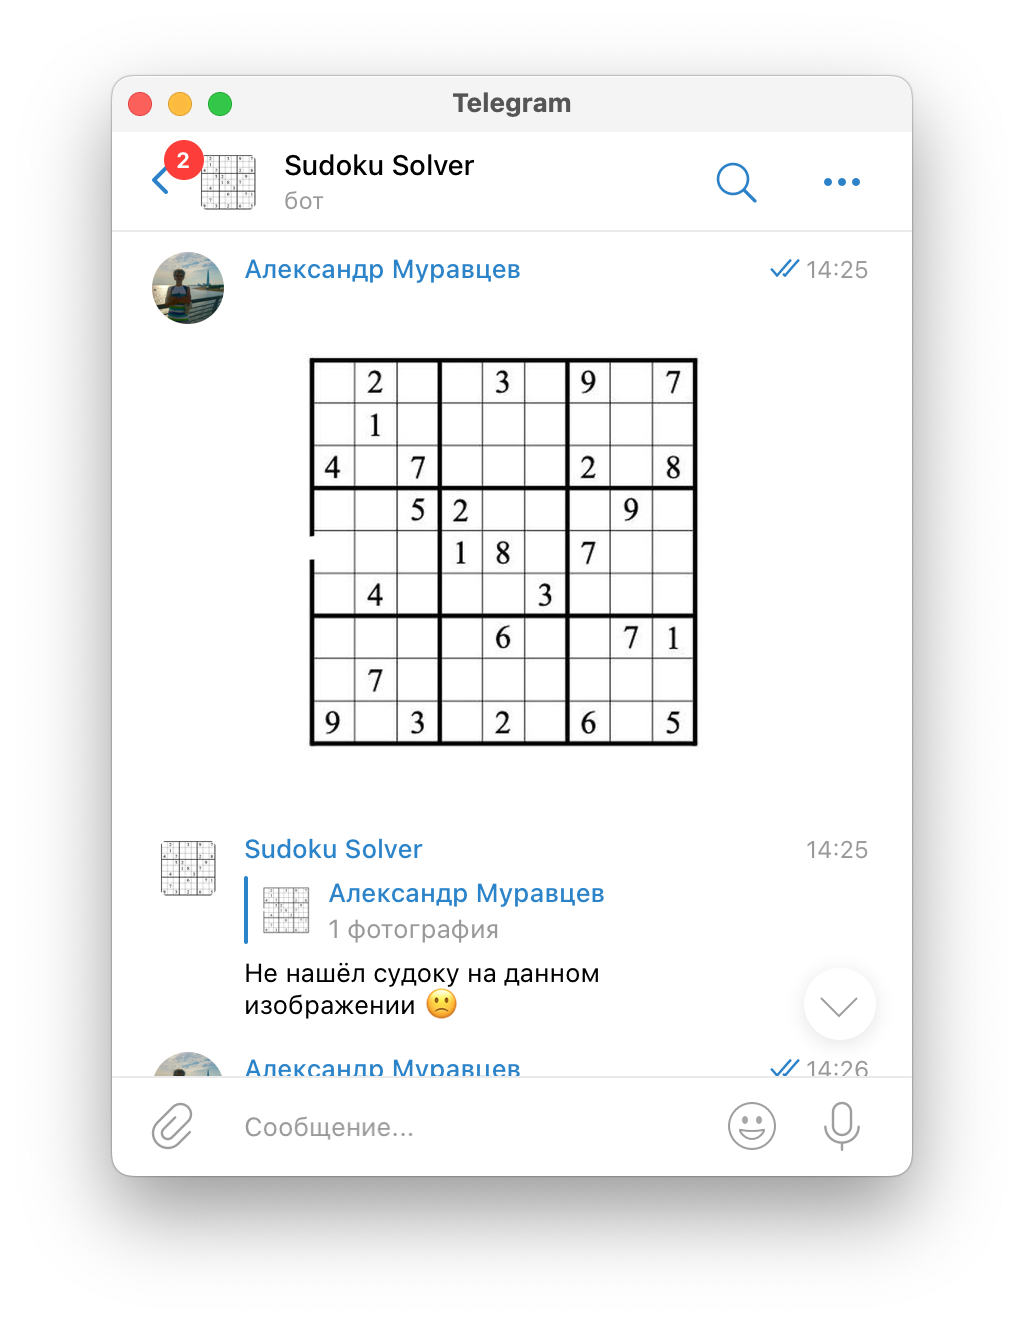
\includegraphics[width=5cm]{telegram_screen_4}
\end{textblock*}

\begin{textblock*}{4.5cm}(8.3cm,1cm)
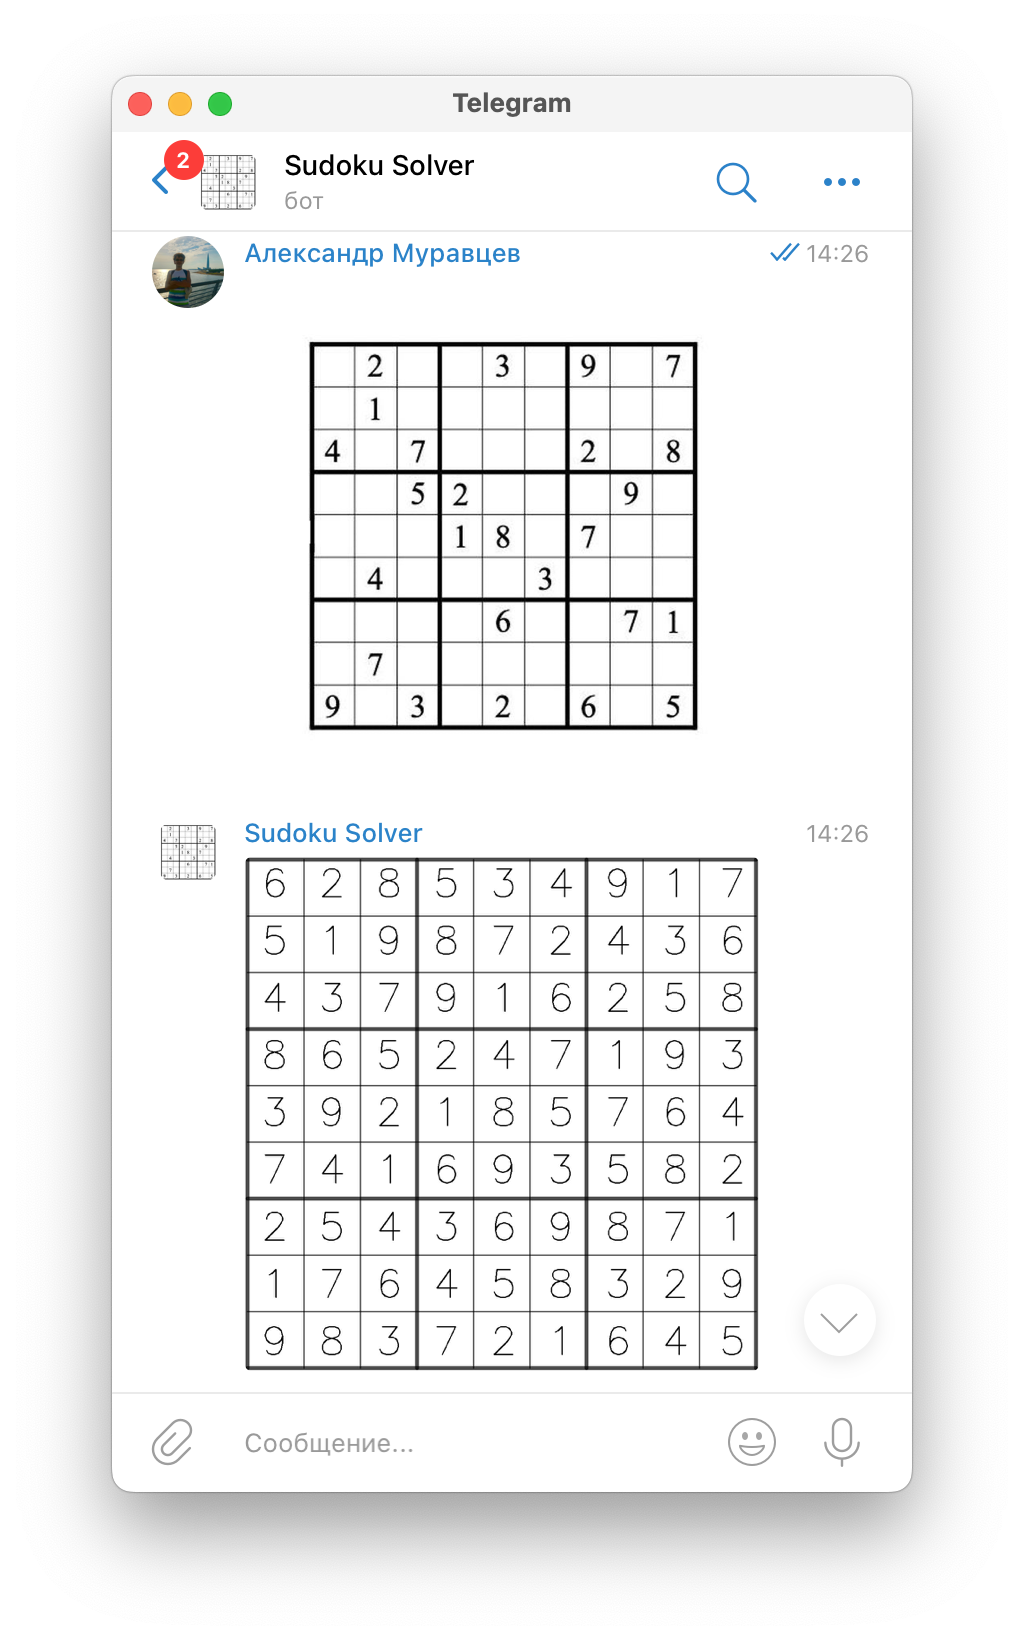
\includegraphics[width=4.5cm]{telegram_screen_5}
\end{textblock*}

\end{frame}



\section{Графическое приложение на PyQT}

\begin{frame}
\frametitle{Интерфейс GUI-приложения}
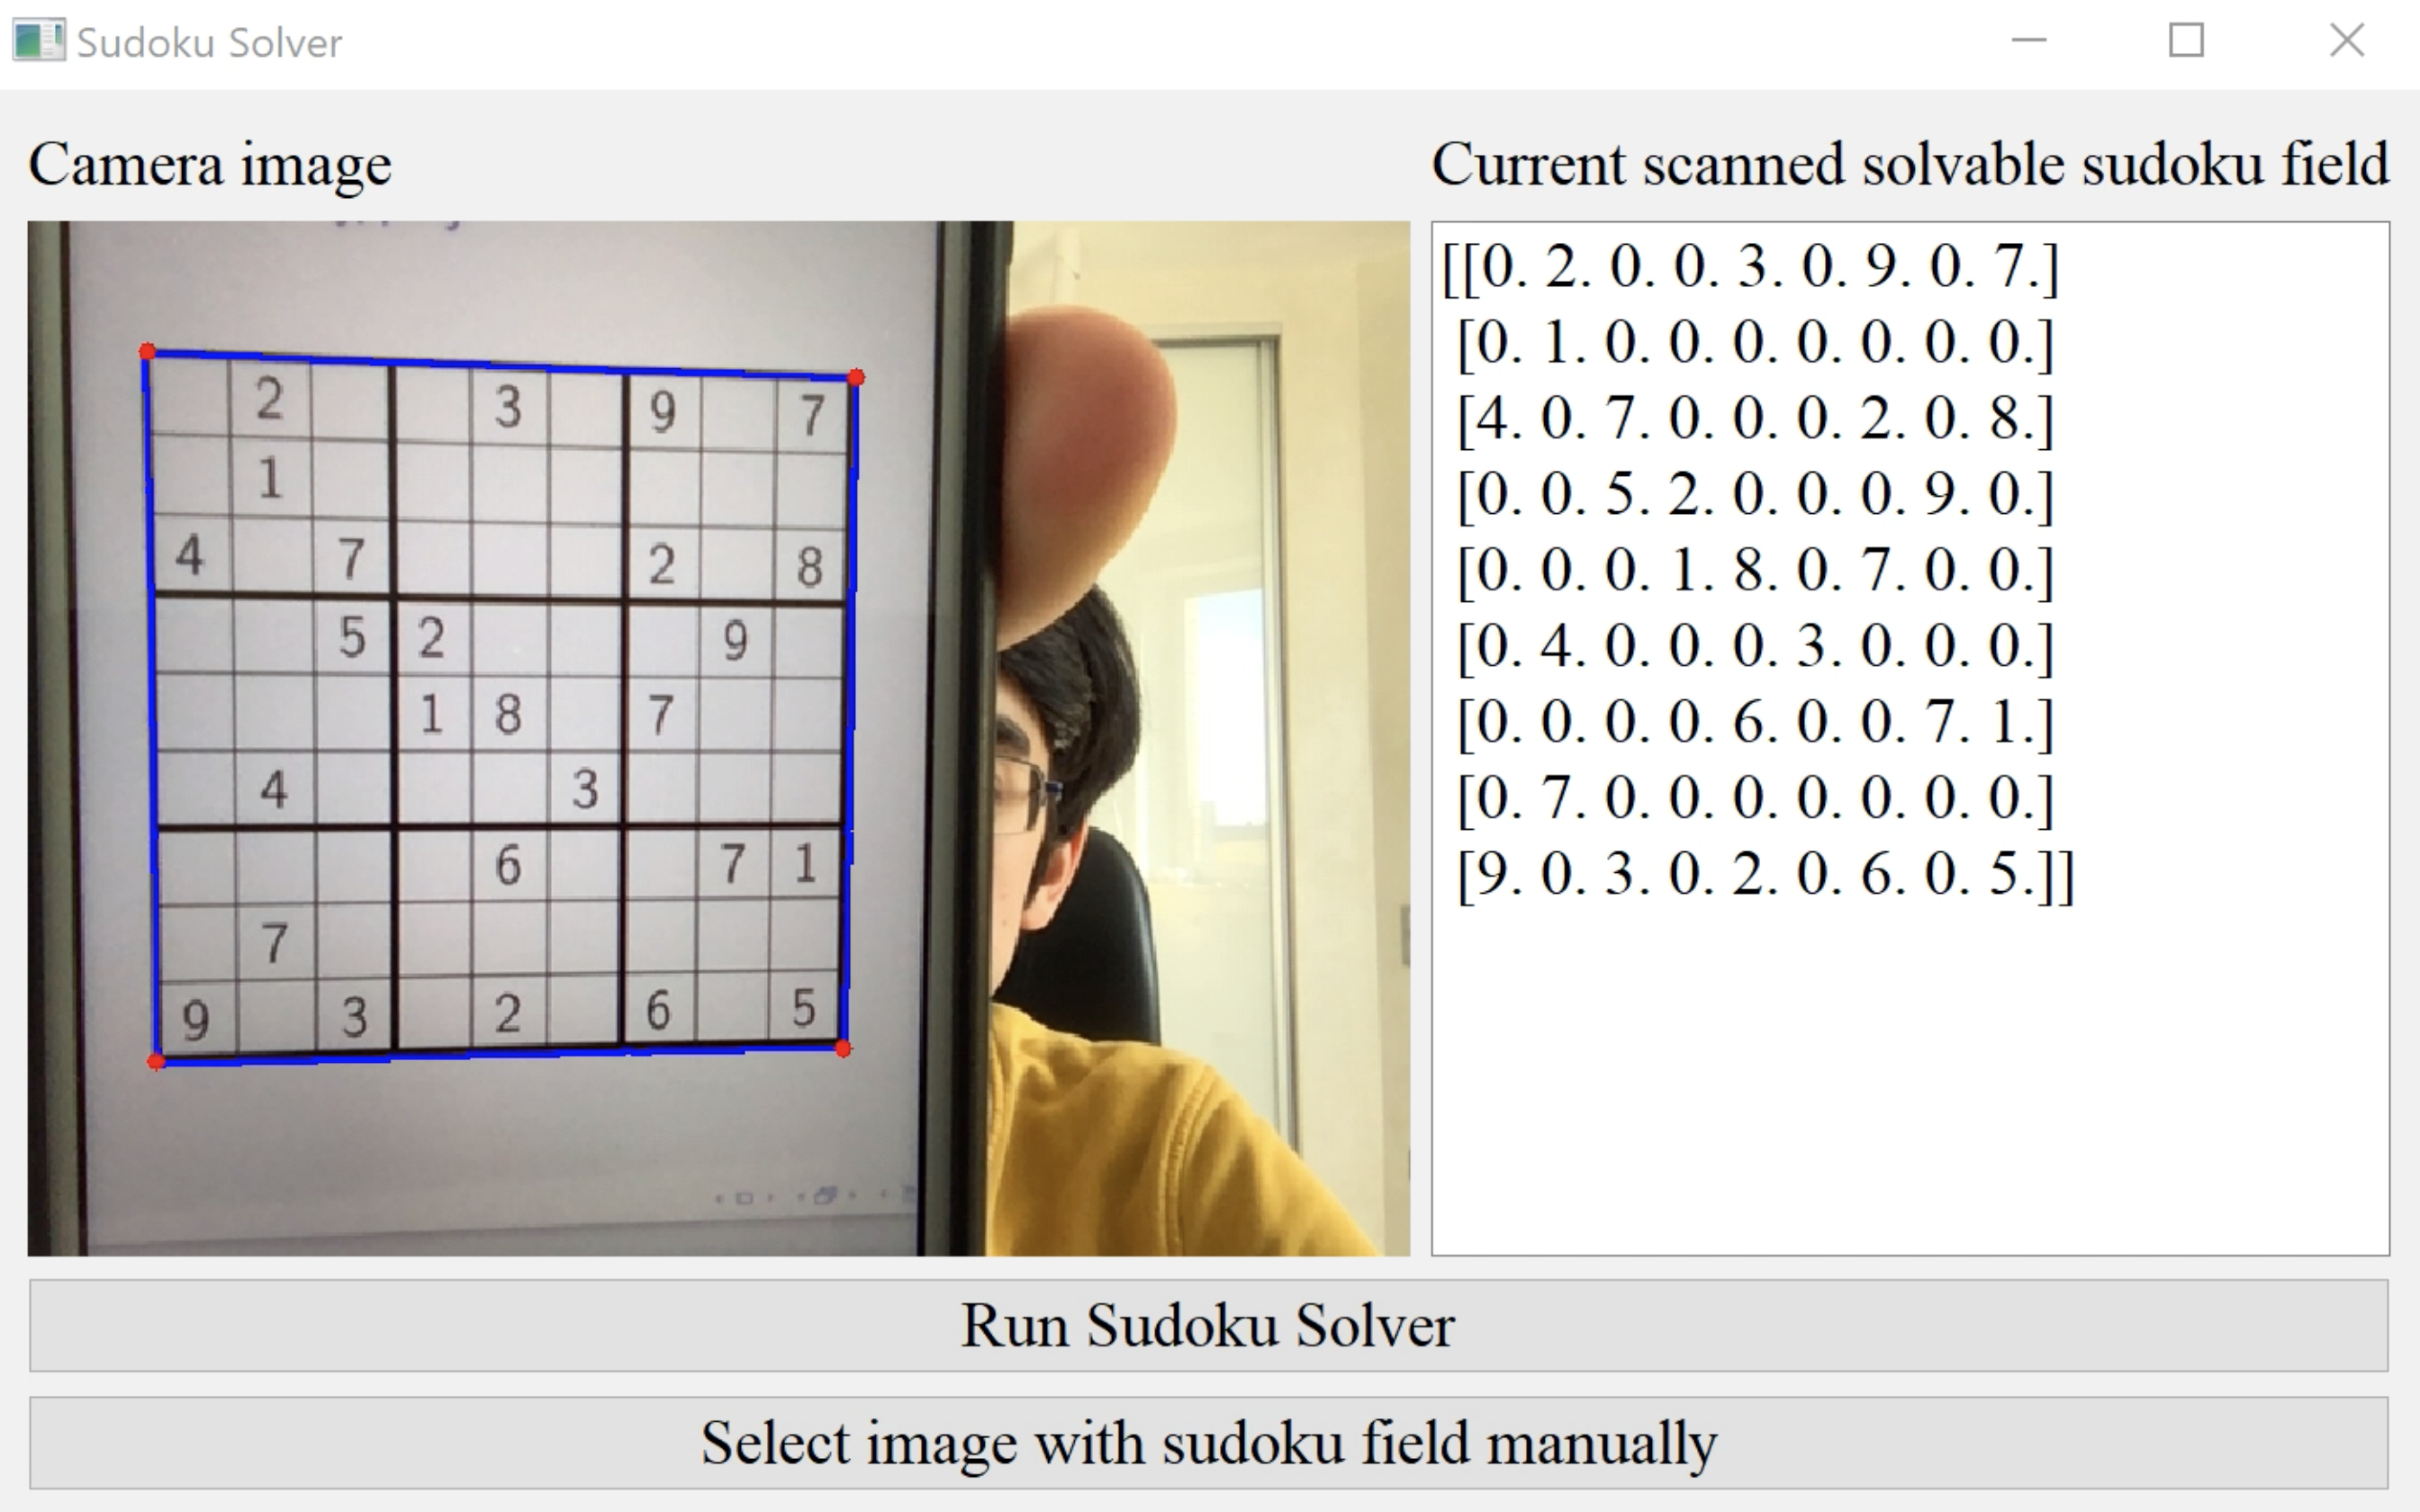
\includegraphics[width=\textwidth]{sudoku_app_in_action}
\end{frame}

\begin{frame}[fragile]
\frametitle{Слоты PyQT}

Слот преобразования openCV изображения в PyQT изображение:
\begin{pythoncode}
    @pyqtSlot(np.ndarray)
    def update_image(self, cv_img):
        """Updates the image_label with a new openCV image"""
        qt_img = self.convert_cv_to_qt(cv_img)
        self.frame_field.setPixmap(qt_img)
\end{pythoncode}
\ \\
Слот обновления текста внутри QTextEdit:
\begin{pythoncode}
    @pyqtSlot(np.ndarray)
    def update_text(self, sudoku_to_solve):
        """Updates the image_label with a new openCV image"""
        self.scanned_sudoku.setText(np.array2string(sudoku_to_solve))
\end{pythoncode}

\end{frame}


\begin{frame}[fragile]
\frametitle{Поток с результатом}
\begin{pythoncode}
class ThreadWithResult(threading.Thread):
    def __init__(self, group=None, target=None, name=None,
                 args=(), kwargs={}, *, daemon=None):
        self.result = None

        def function():
            self.result = target(*args, **kwargs)
        super().__init__(group=group, target=function,
                         name=name, daemon=daemon)
\end{pythoncode}

\begin{textblock*}{8cm}(1cm,2cm)
Класс с выводом результата потока
\end{textblock*}

\begin{textblock*}{10cm}(1cm,7cm)
\footnotesize Создаётся свой поток для каждого из трёх последовательных изображений, полученных с камеры. Если результаты после выполнения каждого из потоков совпадают, то отсканированный судоку записывается в текстовое поле PyQt приложения.
\end{textblock*}

\end{frame}

\section{Возможные пути развития}
\begin{frame}
\frametitle{Возможные пути развития}
Дополнить программу методами сканирования и решения креативных судоку-подобных пазлов:
\begin{itemize}
	\item больших размеров: $16\times16$, \,$12\times12$, \,$25\times25$;
	\item двойные судоку;
	\item чёт-нечёт;
	\item x-судоку; пазл-судоку; виндоку;
	\item судоку больше-меньше;
	\item какуро;
	\item киллер-судоку;
	\item судоку-цветок
\end{itemize}
\ \\
Многие из представленных типов судоку могут быть сведены к задаче о точном покрытии.

\begin{textblock*}{1.5cm}(8.3cm,3.3cm)
\tiny Какуро
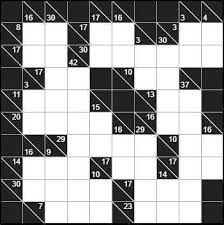
\includegraphics[width=1.5cm]{kakuro.jpg}
\end{textblock*}

\begin{textblock*}{1.5cm}(9.3cm,5.5cm)
\tiny Судоку-цветок
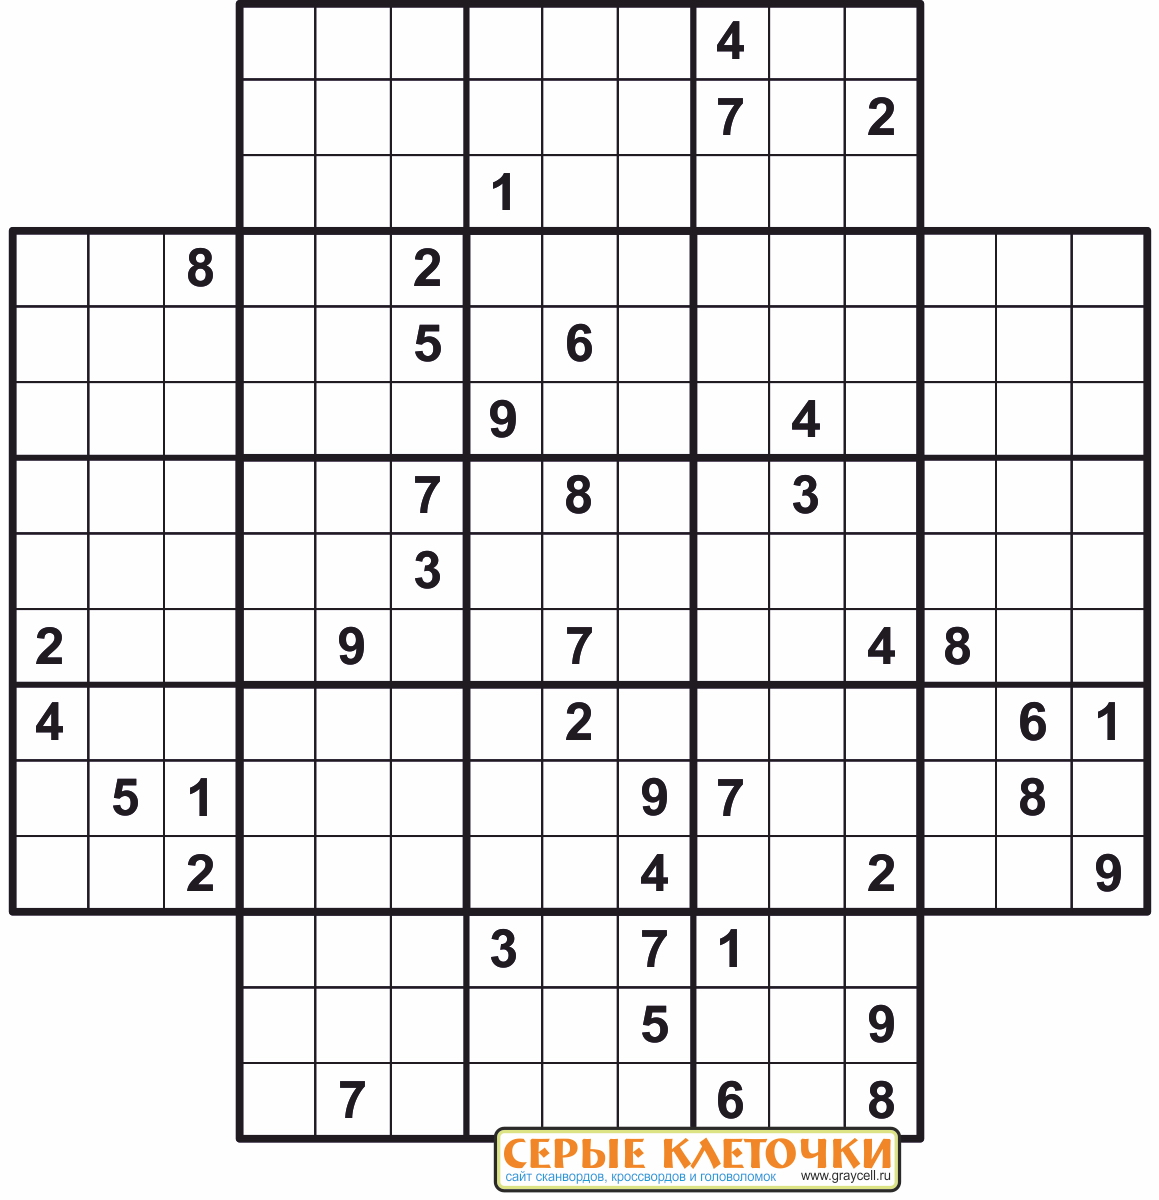
\includegraphics[width=1.5cm]{sudoku_flower}
\end{textblock*}

\begin{textblock*}{1.7cm}(6.5cm,5.55cm)
\tiny Судоку 12 на 12
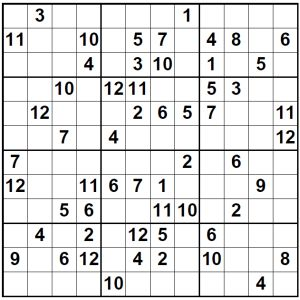
\includegraphics[width=1.7cm]{sudoku12}
\end{textblock*}

\begin{textblock*}{1.8cm}(10.2cm,2.3cm)
\tiny Киллер-судоку
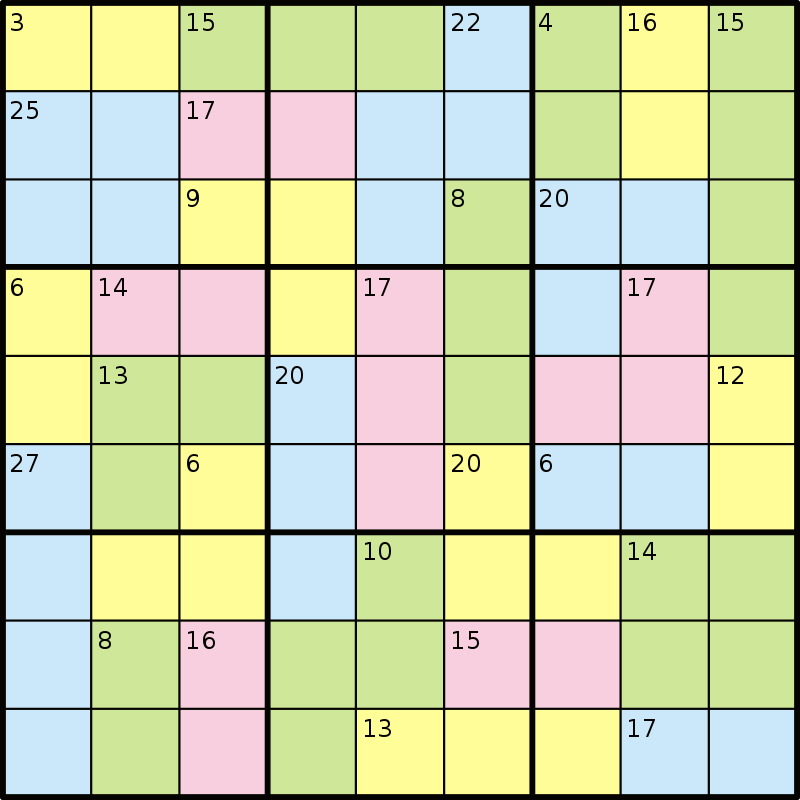
\includegraphics[width=1.8cm]{sudoku_killer}
\end{textblock*}


\end{frame}


\begin{frame}
\frametitle{Возможные пути развития}
Реализовать другой способ взаимодействия пользователя с решателем:
\begin{itemize}
	\item встроить pygame для наглядной визуализации скана судоку;
	\item веб-приложение.
\end{itemize}
\ \\
Запустить собственный генератор классических судоку с заданным уровнем сложности.
\end{frame}


\end{document}
